\documentclass[sigconf]{acmart}

\usepackage{booktabs} % For formal tables

%% -- Local style additions
% \usepackage{times}
\usepackage{xcolor}
\usepackage{siunitx}
\usepackage{multirow}
\usepackage{xspace}
\usepackage{balance}
\usepackage[font=rm]{caption}
\usepackage{algorithm}
\usepackage[noend]{algpseudocode}
\usepackage{verbatim}
\usepackage{graphicx}
\usepackage{tabularx}
\usepackage{enumitem}
\usepackage{shortvrb}
\usepackage{tikz}
\usetikzlibrary{matrix,decorations.pathreplacing,calc,positioning}
\renewcommand{\topfraction}{0.9}
\renewcommand{\bottomfraction}{0.9}
\renewcommand{\textfraction}{0.1}
%% configure number representation defaults
\sisetup{
group-separator = {,},
round-mode = places,
round-precision = 2
}%

\newcommand{\method}[1]{{\small\sf{#1}}}
\newcommand{\gb}[1]{{\mbox{$#1$~GiB}}}
\newcommand{\mb}[1]{{\mbox{$#1$~MiB}}}
\newcommand{\kb}[1]{{\mbox{$#1$~kiB}}}

\newcommand{\tab}{\makebox[2em]{~}}
\newcommand{\var}[1]{\mbox{\emph{#1}}}
\newcommand{\vars}[1]{\mbox{\scriptsize\emph{#1}}}
\newcommand{\sym}[1]{\mbox{\small{\sf{#1}}}}
\newcommand{\syms}[1]{\mbox{\scriptsize{\sf{#1}}}}
\newcommand{\bits}[1]{\mbox{\sf{#1}}}
\newcommand{\BigO}[1]{\ensuremath{O\bigl(#1\bigr)}}
\def\D{\hphantom{1}}
\def\C{\hphantom{1,}}

\newcommand{\myparagraph}[1]{\paragraph*{\hspace*{-\parindent}\normalsize\bf#1.}}
\newcommand{\mycaption}[1]{\caption{{\rm{#1}}}}
\newcommand{\myfootnote}[1]{\footnote{{#1}}}

\usepackage{xcolor}
\newcommand{\jane}[1]{{\color{blue}{\bf{Jane says:}} \emph{#1}}}
\newcommand{\alistair}[1]{{\color{purple}{\bf{Alistair says:}} \emph{#1}}}
\newcommand{\jack}[1]{{\color{orange}{\bf{Jack says:}} \emph{#1}}}
\newcommand{\todo}[1]{{\color{blue}{[[#1]]}}}

\newcommand{\whatever}{\method{WhatEver}}

\newcommand{\collection}[1]{\method{#1}}
\newcommand{\govtwo}{\collection{Gov2}}
\newcommand{\clueweb}{\collection{ClueWeb09}}
\newcommand{\commoncrawl}{\collection{CC}}

\newcommand{\aftertabspace}{\vspace*{-2ex}}
\newcommand{\afterfigspace}{\vspace*{-0ex}}
\newcommand{\afterpixspace}{\vspace*{-1ex}}

\newcommand{\bzip}{{\method{BZip2}}}
\newcommand{\efopt}{\mbox{\method{EF-opt}}}
\newcommand{\ef}{{\method{EF}}}
\newcommand{\interp}{{\method{Interp}}}
\newcommand{\qmx}{\method{QMX}}
\newcommand{\uef}{\method{UEF}}
\newcommand{\ans}{{\method{ANS}}}
\newcommand{\vbyte}{{\method{VByte}}}
\newcommand{\simple}{{\method{Simple}}}
\newcommand{\packed}{{\method{Packed}}}
\newcommand{\pfor}{\method{PFOR}}
\newcommand{\opf}{\method{Opt-PFOR}}
\newcommand{\vbyteplus}{\method{\vbyte+ANS}}
\newcommand{\simpleplus}{\method{\simple+ANS}}
\newcommand{\packedplus}{\method{\packed+ANS}}
\newcommand{\packedpp}{\method{\packed+ANS2}}
\newcommand{\opfplus}{\method{\opf+ANS}}
\newcommand{\ansmapping}{\mbox{\emph{ANSmsb}}}
\newcommand{\xz}{{\method{XZ}}}
\newcommand{\zlib}{{\method{ZLib}}}
\newcommand{\zstd}{{\method{ZStd}}}
\newcommand{\raw}{{\method{U32}}}

\newcommand{\ddt}{{\ensuremath{d_{t,i}}}}
\newcommand{\fdt}{{\ensuremath{f_{t,i}}}}
\newcommand{\dfdt}{{\ensuremath{\langle \ddt, \fdt\rangle}}}

%% -- End local style additions

% Copyright
\setcopyright{none}
%\setcopyright{acmcopyright}
%\setcopyright{acmlicensed}
%\setcopyright{rightsretained}
%\setcopyright{usgov}
%\setcopyright{usgovmixed}
%\setcopyright{cagov}
%\setcopyright{cagovmixed}


% DOI
\acmDOI{10.1145/000000.000000}

% ISBN
\acmISBN{123-4567-24-567/08/06}

%Conference
\acmConference[COMP90049-Knowlege Technologies, University of Melbourne]{August 2017}
\acmYear{2017}
\copyrightyear{2017}

\acmPrice{15.00}

\settopmatter{printacmref=false, printfolios=false}

\begin {document}
\title{Lexical Normalisation of Twitter Data}
%% \titlenote{Produces the permission block, and
%%   copyright information}
%% \subtitle{Extended Abstract}
%% \subtitlenote{The full version of the author's guide is available as
%%   \texttt{acmart.pdf} document}

%% As of 17-06-24 authorship and authorship order not yet discussed.

\author{Siddharth Malhotra}
%% \orcid{1234-5678-9012}
\affiliation{%
  \institution{The University of Melbourne}
}
\email{smalhotra1@student.unimelb.edu.au}


\begin{abstract}
In this report, we discuss two major spelling correction methodologies on the problem of tweet normalisation specifically on Twitter data. Firstly, discuss the combination of Levenshtein Distance, Peter Norwig Algorithm and n-gram context matching, namely LRPN approach. The second method involves first preprocessing the text, tokenisation is performed through NLTK, a lexicon and confusion set is built, scoring and ranking of possible interpretation of Out-of-vocabulary words (OOVs),decoding the confusion lattice thus formed using SRI-LM toolkit, namely NLTK-SRI technique. Further, we perform a critical analysis of these approaches by calculating the $precision$ and $recall$ values.

\end{abstract}




\keywords{Lexical Normalisation; Phonetic Matching; Levenshtein distance; Peter Norvig's Algorithm; N-Gram; NLTK; SRILM}

\maketitle

\begin{abstract}
In this report, we discuss two major spelling correction methodologies on the problem of tweet normalisation specifically on Twitter data. Firstly, discuss the combination of Levenshtein Distance, Peter Norwig Algorithm and n-gram context matching, namely LRPN approach. The second method involves first preprocessing the text, tokenisation is performed through NLTK, a lexicon and confusion set is built, scoring and ranking of possible interpretation of Out-of-vocabulary words (OOVs),decoding the confusion lattice thus formed using SRI-LM toolkit, namely NLTK-SRI technique. Further, we perform a critical analysis of these approaches by calculating the $precision$ and $recall$ values.

\end{abstract}


\section{Introduction}
\label{sec-intro}

Microblogging constitutes the modern method of using social networks. As there is a high input cost associated with using the mobile phone keypads, users tend to shorten their words. 
Twitter, for instance allows 140 or fewer characters, and generally contains hash tags and @ symbols. The proceeding sections describe in detail the various techniques that are applied to
identity: {Known} or {in-vocabulary} words; punctuation and special symbols (both general and Twitter specific); and candidates for normalisation. 
We then apply various normalisation techniques to correct out of vocabulary $OOV$ tokens.










\section{Text Normalisation Techniques}
\label{sec-background}

\subsection{Text Pruning}
Before we begin analysing our tokens, we would want to categorise and extract the tokens which we would want to consider for Normalisation. Our focus is to segregate out tokens into various categories, such as In Vocabulary, Non Candidates and Out of Vocabulary text. We use $labelled-tweets.txt$ for extracting the labelled tokens using $listing.py$. This gives us tokens in a line-by-line format. 


\texttt {\citet{lnt15b}} tokenises and classifies strings into three main categories In-Vocabulary, Out of Vocabulary $($$OOV$$)$ and Non candidate tokens ($NO$). For the purpose of out study, we run a Levenshtein difference analysis using $distance.py$ and place tokens with difference 0 into in-vocabulary terms. The Levenshtein distance is calculated as per the number of substitutions, deletions or additions to be made to the input string to convert the string ${L}$ to ${D}$. 

In order to identify non-candidates (NO), we run a regex string check, on all the terms to classify strings beginning with punctuation symbols, character {\nolinkurl{@}} or \# or http websites using $Outliers.py$. Thus, candidates without the presence of in vocabulary terms and special characters are marked as candidates for lexical normalisation and are termed Out-of-Vocabulary (OOV). 

Usually these are terms that have been misspelt of have been abbreviated in order to fit Twitters 140 character limit. Our $results.txt$ document now contains all the IN and NO words up till this point. For the remaining candidates we perform the normalisation techniques.  \textbf{Table 1} represents the corpura of the words we have used for normalisation. 

\subsection{{\itshape LRPN} Technique}
\begin{table}[t]
\centering

 \begin{tabular}{|c|c|} 
 \hline
 Corpus & Features \\ [0.5ex] 
 \hline\hline
 labelled-tweets.txt & 53KB \\ 
\hline
labelled-tokens.txt & 127KB \\
 \hline
 tokens.txt & 49 KB (8841 words) \\
 \hline
\end{tabular}
\mycaption{Corpura used for Normalisation
\label{tbl-normalize}}
\aftertabspace
\end{table}
  
 \textbf{Normalisation Process:}
  
\textbf{Calculating Edit Distance:} First, the terms with edit distance of 2 are identified and results are stored in an array. These contain words based textual similarity. For this, we use the python-Levenshtein 0.12.0 package. The phrase edit distance is used 
  to refer specifically to Levenshtein distance.The dictionary terms (dict.txt) is searched for matches based on Levenshtein Distance. We perform this step through $distance.py$ and segregate our input token strings $dictionary words$ and $non dictionary$ words. 
  
 \textbf {Note:} Although it is possible to retrace the dictionary words corresponding to the lowest value of the edit distance, we take a conscious decision, based on evaluation of several edit distance measures (global and local) on not doing so as the accuracy of these words extracted will not be optimal in most cases. Subsequently, we combine several techniques to approach the same.
    
\textbf{Peter Norvig's Algorithm:} {\citet{pn15}} introduced an algorithm for the approximate matches. This returns one match deemed closest to the query by the algorithm. Peter Norwig's algorithm considers corrections that require two simple edits. The following steps are performed: Selection Mechanism, Candidate Model, Language Model and Error Model. We use $PeterNorwig.py$ for evaluating the Peter Norwig correction. We combine Peter Norvig with N-gram context matching for increasing the accuracy of normalisation.
  
\textbf{N-gram matching:} $n-gram$ is a contiguous sequence of n items is analysed from a given sequence of text or speech. An n-gram of size 1 is referred to as a "unigram"; size 2 is a "bigram" (or, less commonly, a "digram"); size 3 is a "trigram". Larger sizes are sometimes referred to by the value of n in modern language, e.g., "four-gram", "five-gram", and so on. 
   
   
For each of the OOV's we run different $n-gram$ values from $N=1$ to $N=5$ values using ${generate}\textunderscore{resultsimilarity}.py$. We do this as n-gram may not give us the appropriate string match for lower values of ngram. Through this we analyse the best  ngram decimal values we have obtained for each of the OOV tokens and use ${gen}\textunderscore {nresult.py}$, to pull out the highest ngram value corresponding to each word. For instance, say the OOV word 'commig', the value we get for $N=1$ is $0.875000000$ and the value for $N=2$ is $0.888888889$.

We further maintain a list of all the best N-values for each word and maintain a 
count using ${gennhighest.py}$. From this we make a deduction to find what is the most occurring value of N, giving us the highest results and we further use our chosen N-value to backtrack the possible dictionary word. We use ${gen}
\textunderscore{correspondword.py}$ for getting the possible dictionary word.

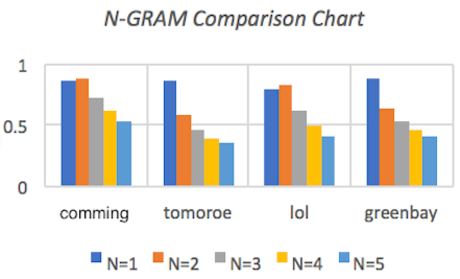
\includegraphics {finalgraph4.pdf}
   
\subsection{{\itshape NLTK-SRI} Technique}

{\citet{gmctw14}} first conduct a context free analysis (at the linguistic level) of all the non-English words. Thus terms such as '2day', 'today' are consider distinct words. Next, they perform normalisation on the noisy text to recover the surface form of the message and record the contextual dimensions, such as, client and location. A text cleaner is built to handle morphophonemic variations. The cleanser marks @username with *USR* and hashtags that are preceded before the end of messages are removed. Hashtags within the middle of the word are removed.

Next, NLTK tokeniser is used to split all tokens that include punctuation symbols. (\textbackslash$w$\text{*}) $($$[$ $P$$]$$)$ (\textbackslash$w$\text{*}) $\rightarrow$ $[$\textbackslash$1$,\textbackslash$2$,\textbackslash$3$$]$ can be used for the same. A confusion network $CN$ is built by comparing token to the words in lexicon $L$. All the tokens be it $IN$ or $OOV$ or punctuation is added tot the CN with probability 1.0. Under the data directory $common\textunderscore abbrs.csv$ maintain a for optimising referencing. A transliteration look up table is built to convert text such as 't0day' $\rightarrow$ ['t0day','today'],refer \textbf{Table 2}. Ranking is performed through a heuristic function (sim()) for each candidate word. 

Confusion Set that is produced this way is joined with the previous set. Finally, lattice is decodes with the use of probabilistic finite state grammar format. At this point, SRI-LM's $lattice-tool$ is used to find the best path through the lattice and training of the set is done as follows. For selecting clean tweets, the following measure was used. Lastly, training of 30M words is done on this set.

\begin{equation}
\label{eq:pr}
\frac{\mathit{Number\ of\ OOV}}{\mathit{Number\ of\ IV+1}} < P ; where P=0.5.
\end{equation}


\begin{table}[t]
\centering

 \begin{tabular}{c c c c} 
 \hline
 Character & Transliteration candidates \\ [0.5ex] 
 \hline\hline
 1 & '1','1','one' \\ 

 2 & '2','to','too','two' \\

 3 & '3','e','three'\\

 4 & '4','a','for','four' \\
 
 5 & '5','s','five' \\ 

 6 & '6','b','six' \\

 7 & '7','t','seven'\\

 8 & '8','ate','eight' \\
 
 9 & '9','g','nine' \\ 

 0 & '0','o','zero' \\

 '@' & '@','at'\\

 "\&" & '\&','and' \\

 \hline
\end{tabular}
\mycaption{Transiliteration lookup table
\label{tbl-normalize}}
\aftertabspace
\end{table}
  










  


\section{Comparison and Review}
\label{sec-somethingnew}

Precision is computed as in equation \eqref{eq:precision}.

\begin{equation}
\label{eq:precision}
Precision = \frac{\mathit{Number\ of\ correct\ predictions}}{\mathit{Total\ number\ of\ predictions}}
\end{equation}

Recall is computed as in equation \eqref{eq:recall}.

\begin{equation}
\label{eq:recall}
Recall = \frac{\mathit{Number\ of\ correct\ words}}{\mathit{Total\ number\ of\ words}}
\end{equation}


\myparagraph{LRPN Technique} Major disadvantage of LRPN strategy is execution cost is quite high. The combination of these strategies provides a much better result than when these are run in a standalone manner.

Using the edit distance, we are able to find out that there are 6652 dictionary words of the 8841 tokens. We are also able to eliminate the non candidate words which are 533. Using Peter Norwig's algorithm we were able to increase the accuracy. Through n-gram technique we found that n=1 and n=2 were of our purpose, thus we made 3312 predictions. In total, 351 words were correctly predicted these techniques. Note: We include the dictionary and non candidate words in the total prediction count. Thus, the total number of predictions adds up to 10497 and correct predictions and the number of correct predictions are 7536.

\begin{equation}
\label{eq:pre}
Precision = \frac{\mathit{Number\ of\ correct\ predictions}}{\mathit{Total\ number\ of\ predictions}} = \frac{\mathit{7536}}{\mathit{10497}} ={{71.8}}
\end{equation}

\begin{equation}
\label{eq:rec}
Recall = \frac{\mathit{Number\ of\ correct\ words}}{\mathit{Total\ number\ of\ words}} = \frac{\mathit{7536}}{\mathit{8841}} ={{85.2}}
\end{equation}
  
\myparagraph{NLTK-SRI Technique} Substantially faster than a LRPN Technique for resolving non candidate words. Also gives a substantial increase in the accuracy.  Certain simple rules can we used to clean up the OOV words, but noisy text cleanser is useful to correct long tail of OOV's. Note: For each word, there are approximately 10 predictions thus making the file and computation size. We have scaled down this analysis to two-thirds of the token file. 

\begin{equation}
\label{eq:prec}
Precision = \frac{\mathit{Number\ of\ correct\ predictions}}{\mathit{Total\ number\ of\ predictions}} = \frac{\mathit{5432}}{\mathit{67390}} ={{8.06}}
\end{equation}


Although the number of correct predictions are high, the number of predictions is large is.number. 

\begin{equation}
\label{eq:recc}
Recall = \frac{\mathit{Number\ of\ correct\ words}}{\mathit{Total\ number\ of\ words}} = \frac{\mathit{5432}}{\mathit{6739}} ={{80.6}}
\end{equation}
\\
The accuracy of NLTK-SRI technique is always above {90\%}.
An Example (from result.txt in TextCleanser-master), if the input is 'wooow of course , i shoulda known that was comingg', the output is 'wow of course, i should known that was coming'.   






%\section{Experiments}
\label{sec-experiments}

\todo{Where much of the hard work is}

Down, down, down.
There was nothing else to do, so Alice soon began talking again.
'Dinah'll miss me very much to-night, I should think!'
(Dinah was the cat.)
'I hope they'll remember her saucer of milk at tea-time.
Dinah my dear!
I wish you were down here with me!
There are no mice in the air, I'm afraid, but you might catch a bat,
and that's very like a mouse, you know.
But do cats eat bats, I wonder?'
And here Alice began to get rather sleepy, and went on saying to
herself, in a dreamy sort of way, 'Do cats eat bats?
Do cats eat bats?'
and sometimes, 'Do bats eat cats?'
for, you see, as she couldn't answer either question, it didn't much
matter which way she put it.
She felt that she was dozing off, and had just begun to dream that
she was walking hand in hand with Dinah, and saying to her very
earnestly, 'Now, Dinah, tell me the truth: did you ever eat a bat?'
when suddenly, thump!
thump!
down she came upon a heap of sticks and dry leaves, and the fall was
over.

Alice was not a bit hurt, and she jumped up on to her feet in a
moment: she looked up, but it was all dark overhead; before her was
another long passage, and the White Rabbit was still in sight,
hurrying down it.
There was not a moment to be lost: away went Alice like the wind, and
was just in time to hear it say, as it turned a corner, 'Oh my ears
and whiskers, how late it's getting!'
She was close behind it when she turned the corner, but the Rabbit
was no longer to be seen: she found herself in a long, low hall,
which was lit up by a row of lamps hanging from the roof.

There were doors all round the hall, but they were all locked; and
when Alice had been all the way down one side and up the other,
trying every door, she walked sadly down the middle, wondering how
she was ever to get out again.


%\section{Conclusions}
\label{sec-conclusions}

Suddenly she came upon a little three-legged table, all made of solid
glass; there was nothing on it except a tiny golden key, and Alice's
first thought was that it might belong to one of the doors of the
hall; but, alas!
either the locks were too large, or the key was too small, but at any
rate it would not open any of them.
However, on the second time round, she came upon a low curtain she
had not noticed before, and behind it was a little door about fifteen
inches high: she tried the little golden key in the lock, and to her
great delight it fitted!

Alice opened the door and found that it led into a small passage, not
much larger than a rat-hole: she knelt down and looked along the
passage into the loveliest garden you ever saw.
How she longed to get out of that dark hall, and wander about among
those beds of bright flowers and those cool fountains, but she could
not even get her head through the doorway; 'and even if my head would
go through,' thought poor Alice, 'it would be of very little use
without my shoulders.
Oh, how I wish I could shut up like a telescope!
I think I could, if I only knew how to begin.'
For, you see, so many out-of-the-way things had happened lately, that
Alice had begun to think that very few things indeed were really
impossible.

There seemed to be no use in waiting by the little door, so she went
back to the table, half hoping she might find another key on it, or
at any rate a book of rules for shutting people up like telescopes:
this time she found a little bottle on it, ('which certainly was not
here before,' said Alice,) and round the neck of the bottle was a
paper label, with the words 'DRINK ME' beautifully printed on it in
large letters.

It was all very well to say 'Drink me,' but the wise little Alice was
not going to do THAT in a hurry. 'No, I'll look first,' she said, 'and
see whether it's marked "poison" or not'; for she had read several nice
little histories about children who had got burnt, and eaten up by wild
beasts and other unpleasant things, all because they WOULD not remember
the simple rules their friends had taught them: such as, that a red-hot
poker will burn you if you hold it too long; and that if you cut your
finger VERY deeply with a knife, it usually bleeds; and she had never
forgotten that, if you drink much from a bottle marked 'poison,' it is
almost certain to disagree with you, sooner or later.

However, this bottle was NOT marked 'poison,' so Alice ventured to
taste it, and finding it very nice, (it had, in fact, a sort of mixed
flavour of cherry-tart, custard, pine-apple, roast turkey, toffee,
and hot buttered toast,) she very soon finished it off.


%-------------------------------------------------------------------%



\balance %% <- doesn't work with footnotes
%% \bibliographystyle{ACM-Reference-Format}
\bibliographystyle{abbrvnat}
\bibliography{strings-shrt,local} 

\end{document}
